\subsection{Mode C Correct}
\label{sec:eval_req_mc_correct} 

\subsubsection{Configuration}

\begin{figure}[H]
    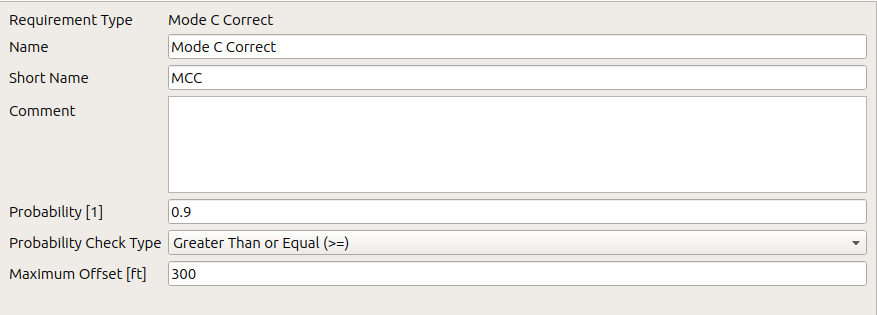
\includegraphics[width=14cm,frame]{figures/eval_req_mc_correct.png}
  \caption{Evaluation Mode C Correct requirement}
\end{figure}

The 'Mode C Correct' requirement is used to calculate the probability of a target report having a correct and valid Mode C code. 
Correct in this context means there is Mode C information data available, and it is the same as in the reference (within a certain threshold). Only values which are valid and not garbled are used. \\

\begin{itemize}  
\item Probability [1]: Probability of correct Mode C code
\item Probability Check Type: $\geq$
\item Maximum Offset [ft]: Maximum absolute distance between reference and test value to be counted as correct
\end{itemize}
\ \\

\subsubsection{Result Values}

\paragraph{Sector}

\begin{center}
 \begin{table}[H]
  \begin{tabularx}{\textwidth}{ | l | X |  l | }
    \hline
    \textbf{Name} & \textbf{Description} & \textbf{Example} \\ \hline
    Sector Layer & Name of the sector layer & fir\_body\_cut \\ \hline
    Requirement Group & Name of the requirement group & Mandatory \\ \hline
    Requirement & Name of the requirement & Mode C Correct \\ \hline
    Num Results & Total number of results & 317 \\ \hline
    Num Usable Results & Number of usable results & 84 \\ \hline
    Num Unusable Results & Number of unusable results & 233 \\ \hline
    \#Updates & Total number target reports & 86477 \\ \hline
    \#NoRef [1] & Number of updates w/o reference position or Mode C & 26095 \\ \hline
    \#NoRefPos [1] & Number of updates w/o reference position  & 26095 \\ \hline
    \#NoRef [1] & Number of updates w/o reference Mode C & 0 \\ \hline
    \#PosInside [1] & Number of updates inside sector & 33243 \\ \hline
    \#PosOutside [1] & Number of updates outside sector & 27139 \\ \hline
    \#CMC [1] & Number of updates with correct Mode C & 33207 \\ \hline
    \#NCMC [1] & Number of updates with no correct Mode C & 36 \\ \hline
    PC [\%] & Probability of correct Mode C & 99.89 \\ \hline
    Condition &  & >= 90.00 \\ \hline
    Condition Fulfilled &  & Passed \\ \hline
\end{tabularx}
\end{table}
\end{center}

Also, a table is given for all single targets, sorted by PC.

\paragraph{Single Target}

\begin{center}
 \begin{table}[H]
  \begin{tabularx}{\textwidth}{ | l | X |  l | }
    \hline
    \textbf{Name} & \textbf{Description} & \textbf{Example} \\ \hline
    Use & To be used in results & true \\ \hline
    \#Up [1] & Number of updates & 1110 \\ \hline
    \#NoRef [1] & Number of updates w/o reference position or Mode C & 1 \\ \hline
    \#NoRefPos [1] & Number of updates w/o reference position  & 1 \\ \hline
    \#NoRef [1] & Number of updates w/o reference Mode C & 0 \\ \hline
    \#PosInside [1] & Number of updates inside sector & 200 \\ \hline
    \#PosOutside [1] & Number of updates outside sector & 909 \\ \hline
    Max Dist. [ft] & Maximum offset & 300.00 \\ \hline
    \#CMC [1] & Number of updates with correct Mode C & 198 \\ \hline
    \#NCMC [1] & Number of updates with no correct Mode C & 2 \\ \hline
    PC [\%] & Probability of correct Mode C & 99 \\ \hline
    Condition &  & >= 90.00 \\ \hline
    Condition Fulfilled &  & Passed \\ \hline
\end{tabularx}
\end{table}
\end{center}

\subsection{Mode C Correct Periods}
\label{sec:eval_req_mc_correct_periods} 

\subsubsection{Configuration}

\begin{figure}[H]
    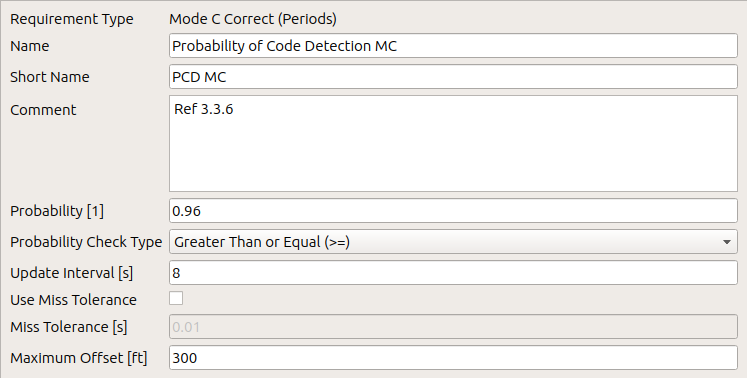
\includegraphics[width=14cm,frame]{figures/eval_req_mc_correct_periods.png}
  \caption{Evaluation Mode C Correct Periods requirement}
\end{figure}

This requirement calculates the probability of correct Mode C detection. \\

For each target existing in the reference data (within the current sector) a test target's Mode C code should
be detected correctly within each test update interval. Correctly here means up to a certain configurable threshold.
Update intervals without correct Mode C code are counted as misses, which are used to calculate the probability of correct Mode C
detection, which has to fulfill a given threshold.

\begin{itemize}  
    \item Probability [1]: Probability of correct Mode C code detection
    \item Probability Check Type: $\geq$
    \item Update Interval [s]: Update interval of the test data
    \item Use Miss Tolerance: Checkbox if miss tolerance should be used
    \item Miss Tolerance [s]: Acceptable time delta for miss detection
    \item Maximum Offset [ft]: Maximum absolute distance between reference and test value for Mode C code to be counted as correct
\end{itemize}

\subsubsection{Result Values}

\paragraph{Sector}

\begin{center}
 \begin{table}[H]
  \begin{tabularx}{\textwidth}{ | l | X |  l | }
    \hline
    \textbf{Name} & \textbf{Description} & \textbf{Example} \\ \hline
    Sector Layer & Name of the sector layer & fir\_body\_cut \\ \hline
    Requirement Group & Name of the requirement group & En-Route \\ \hline
    Requirement & Name of the requirement & Probability of Code Detection MC \\ \hline
    Num Results & Total number of results & 317 \\ \hline
    Num Usable Results & Number of usable results & 81 \\ \hline
    Num Unusable Results & Number of unusable results & 236 \\ \hline
    \#Updates/\#EUIs [1] & Total number update intervals & 4265 \\ \hline
    \#MUIs [1] & Number of missed update intervals & 0 \\ \hline
    PCMCD [\%] & Probability of Correct Mode C Detection & 100.00 \\ \hline
    Condition &  & >= 96.00 \\ \hline
    Condition Fulfilled &  & Passed \\ \hline
    \#Single Targets &  & 81 \\ \hline
    \#Failed Single Targets &  & 0 \\ \hline
\end{tabularx}
\end{table}
\end{center}

\paragraph{Single Target}

\begin{center}
 \begin{table}[H]
  \begin{tabularx}{\textwidth}{ | l | X |  l | }
    \hline
    \textbf{Name} & \textbf{Description} & \textbf{Example} \\ \hline
    Use & To be used in results & true \\ \hline
    \#EUIs [1] & Expected Update Intervals & 12 \\ \hline
    \#MUIs [1] & Missed Update Intervals & 0 \\ \hline
    PCMCD [\%] & Probability of Correct Mode C Detection & 100 \\ \hline
    Reference Period 1 & Time inside sector & [2023-06-30 16:06:17.256,2023-06-30 16:07:56.984] \\ \hline
    Condition &  & >= 96.00 \\ \hline
    Condition Fulfilled &  & Passed \\ \hline
\end{tabularx}
\end{table}
\end{center}

\subsection{Mode C False}
\label{sec:eval_req_mc_false} 

\subsubsection{Configuration}

\begin{figure}[H]
    \includegraphics[width=14cm,frame]{figures/eval_req_mc_false.png}
  \caption{Evaluation Mode C False requirement}
\end{figure}

The 'Mode C False' requirement is used to calculate the probability of a target report having a false Mode C code. False in this context means there is Mode C information data available, and the absolute difference between the test and the reference is larger than the given threshold. \\

\begin{itemize}  
\item Probability [1]: Probability of false Mode C code
\item Probability Check Type: $\leq$
\item Maximum Difference [ft]: Maximum altitude difference between the test and the reference, in feet
\end{itemize}
\ \\

\subsubsection{Result Values}

\paragraph{Sector}

\begin{center}
 \begin{table}[H]
  \begin{tabularx}{\textwidth}{ | l | X |  l | }
    \hline
    \textbf{Name} & \textbf{Description} & \textbf{Example} \\ \hline
    Sector Layer & Name of the sector layer & fir\_cut\_sim \\ \hline
    Requirement Group & Name of the requirement group & Mandatory \\ \hline
    Requirement & Name of the requirement & Mode C False \\ \hline
    Num Results & Total number of results & 728 \\ \hline
    Num Usable Results & Number of usable results & 107 \\ \hline
    Num Unusable Results & Number of unusable results & 621 \\ \hline
    Use & To be used in results & true \\ \hline
    \#Up [1] & Number of updates & 101685 \\ \hline
    \#NoRef [1] & Number of updates w/o reference position or code & 7363 \\ \hline
    \#NoRefPos [1] & Number of updates w/o reference position  & 7359 \\ \hline
    \#NoRef [1] & Number of updates w/o reference code & 4 \\ \hline
    \#PosInside [1] & Number of updates inside sector & 53997 \\ \hline
    \#PosOutside [1] & Number of updates outside sector & 40329 \\ \hline
    \#Unknown [1] & Number of updates unknown code & 40 \\ \hline
    \#Correct [1] & Number of updates with correct code & 53935 \\ \hline
    \#False [1] & Number of updates with false code & 18 \\ \hline
    PF [\%] & Probability of Mode C false & 0.03 \\ \hline
    Condition &  & <= 3.00 \\ \hline
    Condition Fulfilled &  & Passed \\ \hline
\end{tabularx}
\end{table}
\end{center}

Also, a table is given for all single targets, sorted by PF.

\paragraph{Single Target}

\begin{center}
 \begin{table}[H]
  \begin{tabularx}{\textwidth}{ | l | X |  l | }
    \hline
    \textbf{Name} & \textbf{Description} & \textbf{Example} \\ \hline
    Use & To be used in results & true \\ \hline
    \#Up [1] & Number of updates & 709 \\ \hline
    \#NoRef [1] & Number of updates w/o reference position or code & 30 \\ \hline
    \#NoRefPos [1] & Number of updates w/o reference position  & 30 \\ \hline
    \#NoRef [1] & Number of updates w/o reference code & 0 \\ \hline
    \#PosInside [1] & Number of updates inside sector & 591 \\ \hline
    \#PosOutside [1] & Number of updates outside sector & 88 \\ \hline
    \#Unknown [1] & Number of updates unknown code & 0 \\ \hline
    \#Correct [1] & Number of updates with correct code & 585 \\ \hline
    \#False [1] & Number of updates with false code & 6 \\ \hline
    PF [\%] & Probability of Mode C false & 1.02 \\ \hline
    Condition &  & <= 3.00 \\ \hline
    Condition Fulfilled &  & Passed \\ \hline
\end{tabularx}
\end{table}
\end{center}

\subsection{Mode C Present}
\label{sec:eval_req_mc_present} 

\subsubsection{Configuration}

\begin{figure}[H]
    \includegraphics[width=14cm,frame]{figures/eval_req_mc_present.png}
  \caption{Evaluation Mode C Present requirement}
\end{figure}

The 'Mode C Present' requirement is used to calculate the probability of a target report having any Mode C code. Present in this context means there is Mode C information data available, irrespectively if correct or not. \\

\begin{itemize}  
\item Probability [1]: Probability of Mode C code present
\item Probability Check Type: $\geq$
\end{itemize}
\ \\

\subsubsection{Result Values}

\paragraph{Sector}

\begin{center}
 \begin{table}[H]
  \begin{tabularx}{\textwidth}{ | l | X |  l | }
    \hline
    \textbf{Name} & \textbf{Description} & \textbf{Example} \\ \hline
    Sector Layer & Name of the sector layer & fir\_cut\_sim \\ \hline
    Requirement Group & Name of the requirement group & Mandatory \\ \hline
    Requirement & Name of the requirement & Mode C Present \\ \hline
    Num Results & Total number of results & 728 \\ \hline
    Num Usable Results & Number of usable results & 107 \\ \hline
    Num Unusable Results & Number of unusable results & 621 \\ \hline
    Use & To be used in results & true \\ \hline
    \#Up [1] & Number of updates & 101685 \\ \hline
    \#NoRef [1] & Number of updates w/o reference position & 7359 \\ \hline
    \#NoRefPos [1] & Number of updates w/o reference position  & 7359 \\ \hline
    \#PosInside [1] & Number of updates inside sector & 53997 \\ \hline
    \#PosOutside [1] & Number of updates outside sector & 40329 \\ \hline
    \#NoRefC [1] & Number of updates without reference code & 4 \\ \hline
    \#Present [1] & Number of updates with present tst code & 53953 \\ \hline
    \#Missing [1] & Number of updates with missing tst code & 40 \\ \hline
    PP [\%] & Probability of Mode C present & 99.93 \\ \hline
    Condition &  & >= 97.00 \\ \hline
    Condition Fulfilled &  & Passed \\ \hline
\end{tabularx}
\end{table}
\end{center}

Also, a table is given for all single targets, sorted by PP.

\paragraph{Single Target}

\begin{center}
 \begin{table}[H]
  \begin{tabularx}{\textwidth}{ | l | X |  l | }
    \hline
    \textbf{Name} & \textbf{Description} & \textbf{Example} \\ \hline
    Use & To be used in results & true \\ \hline
    \#Up [1] & Number of updates & 1041 \\ \hline
    \#NoRef [1] & Number of updates w/o reference position & 92 \\ \hline
    \#NoRefPos [1] & Number of updates w/o reference position  & 92 \\ \hline
    \#PosInside [1] & Number of updates inside sector & 406 \\ \hline
    \#PosOutside [1] & Number of updates outside sector & 543 \\ \hline
    \#NoRefC [1] & Number of updates without reference code & 0 \\ \hline
    \#Present [1] & Number of updates with present tst code & 398 \\ \hline
    \#Missing [1] & Number of updates with missing tst code & 8 \\ \hline
    PP [\%] & Probability of Mode C present & 98.03 \\ \hline
    Condition &  & >= 97.00 \\ \hline
    Condition Fulfilled &  & Passed \\ \hline
\end{tabularx}
\end{table}
\end{center}

\subsection{ROCD Correct}
\label{sec:eval_req_rocd_correct} 

\subsubsection{Configuration}

\begin{figure}[H]
    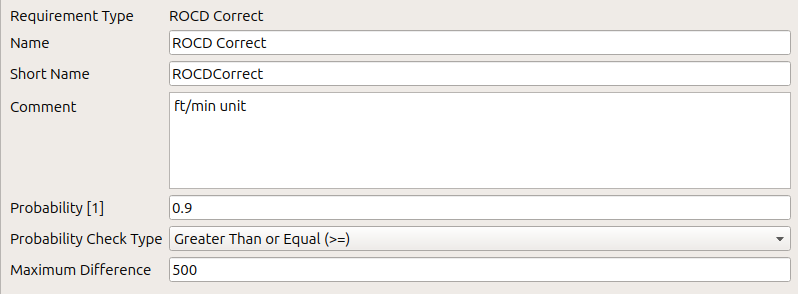
\includegraphics[width=14cm,frame]{figures/eval_req_rocd_correct.png}
  \caption{Evaluation ROCD Correct requirement}
\end{figure}

The 'ROCD Correct' requirement is used to calculate the probability of a target report having an rate of climb/descend error smaller than a defined threshold. The difference of the ROCD (test value vs. linear interpolated reference values) is calculated, and if its absolute value is smaller or equal than the defined threshold, the target report is counted for the calculated probability PCROCD (probability of correct ROCD). The PCROCD must be greater or equal than the defined 'Probability' for the requirement to pass. \\

\begin{itemize}  
\item Probability [1]: Probability of Correct ROCD
\item Probability Check Type: $\geq$
\item Maximum Difference: Maximum ROCD difference between the test and the reference, in feet / minute
\end{itemize}
\ \\

\subsubsection{Result Values}

\paragraph{Sector}

\begin{center}
 \begin{table}[H]
  \begin{tabularx}{\textwidth}{ | l | X |  l | }
    \hline
    \textbf{Name} & \textbf{Description} & \textbf{Example} \\ \hline
    Sector Layer;Name of the sector layer;units\_OPS\_2024 \\ \hline
    Requirement Group & Name of the requirement group & Mandatory \\ \hline
    Requirement & Name of the requirement & ROCD Correct \\ \hline
    Num Results & Total number of results & 1969 \\ \hline
    Num Usable Results & Number of usable results & 1354 \\ \hline
    Num Unusable Results & Number of unusable results & 615 \\ \hline
    Use & To be used in results & true \\ \hline
    \#Up [1] & Number of updates & 580674 \\ \hline
    \#NoRef [1] & Number of updates w/o reference position or Rate of Climb/Descent & 342 \\ \hline
    \#NoRefPos [1] & Number of updates w/o reference position & 149 \\ \hline
    \#NoRef [1] & Number of updates w/o reference Rate of Climb/Descent & 193 \\ \hline
    \#PosInside [1] & Number of updates inside sector & 580230 \\ \hline
    \#PosOutside [1] & Number of updates outside sector & 295 \\ \hline
    \#Unknown [1] & Number of updates unknown Rate of Climb/Descent & 2686 \\ \hline
    \#Correct [1] & Number of updates with correct Rate of Climb/Descent & 470822 \\ \hline
    \#False [1] & Number of updates with incorrect Rate of Climb/Descent & 106529 \\ \hline
    PCROCD [\%] & Probability of Correct ROCD & 81.55 \\ \hline
    Condition &  & >= 90.00 \\ \hline
    Condition Fulfilled &  & Failed \\ \hline
\end{tabularx}
\end{table}
\end{center}

Also, a table is given for all single targets, sorted by PCROCD.

\paragraph{Single Target}

\begin{center}
 \begin{table}[H]
  \begin{tabularx}{\textwidth}{ | l | X |  l | }
    \hline
    \textbf{Name} & \textbf{Description} & \textbf{Example} \\ \hline
    Use & To be used in results & true \\ \hline
    \#Up [1] & Number of updates & 813 \\ \hline
    \#NoRef [1] & Number of updates w/o reference position or Rate of Climb/Descent & 0 \\ \hline
    \#NoRefPos [1] & Number of updates w/o reference position  & 0 \\ \hline
    \#NoRef [1] & Number of updates w/o reference Rate of Climb/Descent & 0 \\ \hline
    \#PosInside [1] & Number of updates inside sector & 813 \\ \hline
    \#PosOutside [1] & Number of updates outside sector & 0 \\ \hline
    \#Unknown [1] & Number of updates unknown Rate of Climb/Descent & 0 \\ \hline
    \#Correct [1] & Number of updates with correct Rate of Climb/Descent & 702 \\ \hline
    \#False [1] & Number of updates with incorrect Rate of Climb/Descent & 111 \\ \hline
    PCROCD [\%] & Probability of Correct ROCD & 86.35 \\ \hline
    Condition &  & >= 90.00 \\ \hline
    Condition Fulfilled &  & Failed \\ \hline
\end{tabularx}
\end{table}
\end{center}
